\section{Property Reification}
\label{sec:Property}
%%%%%%%%%%%%%%%%%%%%%%%%%%%%%%%%%%%%%%%%%%%%%%%%%%%%%%%%
\begin{figure}[h!]
\begin{center}
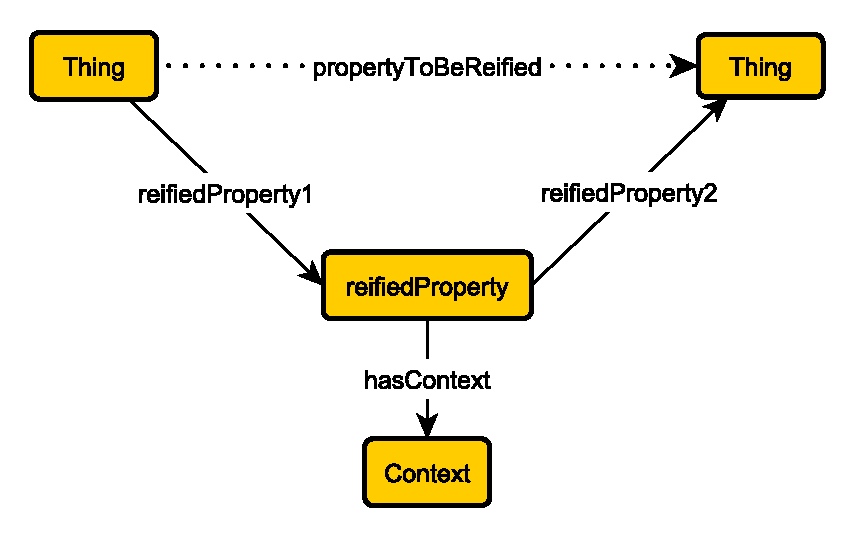
\includegraphics[width=.7\textwidth]{figures/reification}
\end{center}
\caption{Schema Diagram for Property Reification. The visual notation is explained in Chapter \ref{chap:prelims}. Additioanlly, we use the dotted line with solid arrow to indicate which property is being reified. This relation has no bearing on the below axioms.}
\label{fig:Property}
\end{figure}
\subsection{Summary}
\label{sum:Property}
%%%%%%%%%%%%%%%%%%%%%%%%%%%%
In OWL, unfortunately, it is not possible to directly represent $n$-ary relationships. However, it is still possible to capture that information. This notion is called reification. The \textsf{Property Reification} pattern is essentially a metapattern; it could be better considered to be a modelling practice. Here, though, we present a set of axioms that will allow a developer to quickly reify a concept by specializing the framework.

Consider that we would like to relate two \textsf{Things} together via some \textsf{propertyToBeReified} given some \textsf{Context} information that also needs to be captured. To do so, we create a \textsf{ReifiedProperty} and attach the information to this concept. A more concrete example of this can be seen in the \textsf{AgentRole} and \textsf{ParticipantRole} patterns (Sections \ref{sec:AgentRole} and {\ref{sec:ParticipantRole}).

The axioms below are minimalistic, because it is hard to make claims about the domain and range at the most general case. It should be safe to say that there is certain some connection between the first object of interest and the reified property itself. But, perhaps, the second reified property is reused from some other pattern or part of the ontology---we cannot make any statements about it at this level. Furthermore, concept of ``context'' is loose and open to interpretation by the developer. Could it be subclassed during specialization or use of this pattern, perhaps? Is it necessary, perhaps not. It does, however, suffice to show \emph{how} reification with context works.
%%%%%%%%%%%%%%%%%%%%%%%%%%%%%%%%%%%%%%%%%%%%%%%%%%%%%%%%
\subsection{Axiomatization}
\label{axs:Property}
%%%%%%%%%%%%%%%%%%%%%%%%%%%%
\begin{align}
\top &\sqsubseteq \forall \textsf{reifiedProperty1.ReifiedProperty} \\
\top &\sqsubseteq \forall \textsf{hasContext.Context} \\
\top &\sqsubseteq \exists \textsf{hasContext.Context} \\
\end{align}

%%%%%%%%%%%%%%%%%%%%%%%%%%%%%%%%%%%%%%%%%%%%%%%%%%%%%%%%
\subsection{Explanations}
\label{exp:Property}
%%%%%%%%%%%%%%%%%%%%%%%%%%%%
\begin{enumerate}
\item Range: the range of \textsf{reifiedProperty1} is \textsf{ReifiedProperty}.
\item Range: the range of \textsf{hasContext} is \textsf{Context}.
\item Existential: a \textsf{ReifiedProperty} should have at least some contextual information, otherwise, it wouldn't need to be reified.

\end{enumerate}

%%%%%%%%%%%%%%%%%%%%%%%%%%%%%%%%%%%%%%%%%%%%%%%%%%%%%%%%
\subsection{Competency Question}
\label{cqs:Property}
%%%%%%%%%%%%%%%%%%%%%%%%%%%%
\begin{enumerate}[CQ1.]
\item What was the street named during the Great Depression?
\item From what years was Al Gore Vice President?
\item What is the unit of measurement was used to weigh the elephant?
\end{enumerate}

\newpage
%%%%%%%%%%%%%%%%%%%%%%%%%%%%%%%%%%%%%%%%%%%%%%%%%%%%%%%%
% End Section
%%%%%%%%%%%%%%%%%%%%%%%%%%%%%%%%%%%%%%%%%%%%%%%%%%%%%%%%
%%%%%%%%%%%%%%%%%%%%%%%%%%%%%%%%%%%%%%%%%%%%%%%%%%%%%%%%